\chapter{Analyse van de resultaten}\label{sec:analyse}
In dit hoofdstuk worden de observaties in meer detail besproken. Voor elke observatie zal er geprobeerd worden een verklaren te vinden of een hypothese voor te stellen. 

Eerst zal de calibratie aan bod komen, vervolgens de beschikbaarheids- en tenslotte de consistentietesten. Bij elke test zullen eerst de verschillende systemen besproken worden om vervolgens een vergelijking te maken. 

\section{Calibratie}
Over de calibratie testen valt in het algemeen niet veel af te leiden, de verschillende systemen hebben niet hetzelfde aantal instanties, zo heeft Pgpool-II slechts 3 instanties t.o.v. 6 voor MongoDB. 

Enkel op de stijgende variatie van de vertagingen in MongoDB zal dieper ingegaan worden. De reden hiervoor is een lezers/schrijving locking systeem op een gehele database\cite{mongodb-concurrency}. Hierdoor zorgt een leesactie voor de blokkering van alle schrijfactie op de database en vice versa. Naar mate er meer gebruikers zijn, kunnen er meer opeenvolgende schrijfoperaties zijn, dit zal de leesacties langer blokkeren. Maar indien alle gebruikers samen lezen, kan dit parallel gebeuren, een grotere variatie in de vertraging treedt hierdoor op. 

\section{Beschikbaarheidstest}
Bij de beschikbaarheidstesten blijkt er uit de resultaten dat de verschillende systemen een andere aanpak hebben genomen. Voor elk systeem zullen de 3 testen in detail besproken worden, daarna zal een vergelijking tussen de 3 systemen besproken worden. Belangrijk  is dat er hier bewerking aan de basisbelasting uitgevoerd worden, waardoor er data van de verschillende datadistributies gelezen zal worden. 

\paragraph{HBase} Bij HBase heeft een bepaalde RegionServer de verantwoordelijkheid over een Regio voor een bepaalde tijd. Dit is een sessie dit door HMaster uitgedeeld wordt en bijgehouden wordt in Zookeeper. Deze sessie kan vroegtijdig beëindigd worden of er moet gewacht worden tot deze verlopen is, enkel op die momenten kan er een nieuwe RegionServer aangeduid worden. Dit zorgt voor een duidelijk verschil tussen een zachte stop, een harde stop of een netwerk onderbreking. 

De duur van een sessie kan geconfigureerd worden in Zookeeper en staat standaard op 180 seconden. \cite{hbase-doc}. 

\subparagraph{Zachte stop} Bij een zachte stop, is er slechts af en toe sprake dat dit merkbaar is, de verklaring hiervoor is dat dit enkel wordt opgemerkt als de RegionServer die op dat moment verantwoordelijke is voor de Region wordt stopgezet. In de testen is dit niet zichtbaar omdat er verschillende opeenvolgende queries worden uitgevoerd, hierdoor zal data van verschillende regio's gelezen worden tot de blokkerende regio wordt gevonden.  \\
Indien een RegionServer wordt stopgezet, nemen de queries tijdelijk meer tijd in beslag. Na het stopzetten van de RegionServer is er in bepaalde gevallen een verhoogde vertraging in beide leesoperaties (scan en lees). \\
Zodra er een herverdeling is van de Regions over de aanwezige Regionservers, verdwijnt deze verhoogde vertraging. 

\subparagraph{Netwerk onderbreking} Bij een netwerk onderbreking, worden de queries tijdelijk stopgezet en falen de queries in tussentijd. Deze onderbreking duurt significant langer dan in het geval van een zachte stop. Dit komt doordat de regio's pas kunnen toegewezen worden na het verlopen van hun sessie.  

\subparagraph{Harde stop} Bij het stopzetten van een instantie op de harde manier, zijn er twee reacties: de eerste is vergelijkbaar met deze van een netwerk onderbreking. De andere laat pas opnieuw queries toe na het herstellen van het netwerk verkeer. In een manuele test bleek dit opgelost te zijn na het verbreken van de connectie en het opnieuw verbinden, maar de oorzaak waarom dit slecht af en toe voorkomt, is niet gevonden. 

\subparagraph{Herstel van de instantie} Het herstel van de server zal automatisch op een asynchrone manier gebeuren. Er valt te configureren hoeveel data er maximaal per seconde zal worden gesynchroniseerd. Het herstel is niet merkbaar voor de gebruiker bij de testen. 

\paragraph{MongoDB} Bij MongoDB is er tussen de leden van een Replicaset een heartbeat protocol. Indien er gedurende 10 seconden geen antwoord op een een heartbeat komt, wordt een server als offline bestempeld. De server die het laatst een bericht van de primary heeft gekregen zal zijn rol overnemen indien deze uitvalt \cite{mongodb-manual}. Dit heeft zijn invloed op de verschillende manieren om een server stop te stopzetten. 

\subparagraph{Zachte stop en harde stop} Bij een zachte of harde stop is er een kans van 1 op 3 dat het uitvallen van een instantie zichtbaar is, dit is te verklaren doordat enkel het uitschakelen van de primary een invloed zal hebben op de vertraging. In de standaard modus wordt er enkel gelezen naar en geschreven van de primary. Na de verkiezing van een nieuwer primary is er geen verschil in vertraging per soort query ten opzichte van ervoor. Er zijn 2 hypothesen waarom een harde stop op dezelfde manier reageert: bij een harde stop wordt de sessie nog altijd vrijgegeven, of er zijn verkiezingen voor een nieuwe primary voordat de sessie van de oude primary is afgelopen. Deze hypothesen zijn niet getest of verder onderzocht. 

\subparagraph{Netwerk onderbreking} Bij een netwerk onderbreking zou het te verwachten zijn dat na maximaal 10 seconde de primary zou veranderen. Onder de aangelegde belasting blijkt dat de database heel de tijd onbeschikbaar tot de primary opnieuw bereikbaar is via het netwerk. Bij het manueel testen blijkt dat er dezelfde foutmelding gegeven wordt als bij het stoppen van de database, maar dat de data onbeschikbaar is. Het volstaat om de verbindingen af te sluiten en opnieuw aan te maken om het probleem op te lossen. Er is geen reden gevonden voor dit gedrag. 

\subparagraph{Herstel van de instantie} Het herstel van de server zal automatisch op een asynchrone manier gebeuren. Dit is niet merkbaar voor de gebruikers en de server zal als secondary ingezet worden. 

\paragraph{Pgpool-II} Bij Pgpool-II wordt de status van de PostgreSQL instanties getest wanneer er een gebruiker actief is.  Bij het uitvallen van een instantie en opnieuw opstarten terwijl er geen gebruiker verbonden is met Pgpool-II, zal dit niet opgemerkt worden. Daarnaast zijn er verschillende reacties op de geteste scenario's. 

Een vereiste bij het herstellen van een instantie is dat er op dat moment geen enkele verbinding met de router instantie is. 

\subparagraph{Zachte stop} Bij een zachte stop van een data instantie worden alle verbinden van de gebruikers met Pgpool-II onmiddellijk verbroken. Nadien kan er terug verbonden worden met Pgpool-II. In deze omgeving gaan nadien de verschillende schrijfoperaties sneller omdat deze niet meer gerepliceerd moeten worden. Een hypothese is dat bij een grote hoeveelheid data instanties dit effect kleiner zal worden.  

\subparagraph{Harde stop} Een harde stop reageert hetzelfde als een zachte stop. Dit omdat ook hier de connecties onmiddellijk verbroken zijn. Het besturingssysteem van de data instantie zal antwoorden dat er geen service op de poort aan het luisteren is en Pgpool-II detecteert de fout. 

\subparagraph{Netwerk onderbreking} Bij een netwerk onderbreking is er een ander gedrag, de queries wachten op een antwoord maar krijgen dit niet. Hierdoor wordt er gewacht op de time-out die standaard 30 seconde is. Na deze tijd worden connecties verbroken. De gebruiker kan opnieuw verbinden en queries uitvoeren. 

\subparagraph{Vermindering van schrijfvertraging} De reden tot de vermindering van de schrijfvertraging is te vinden in de manier dat Pgpool-II de replicatie van de queries doet. Deze zullen eerst op de master uitgevoerd worden en vervolgens op de slaves. Bij het wegvallen van een instantie is er nog maar een enkele data server over, hierdoor duurt een schrijfactie maar half zo lang. De leesacties duren ongeveer even lang aangezien dezelfde acties nog steeds genomen worden. 

\subparagraph{Herstel van de instantie} Bij het opnieuw inschakelen van een instantie dient in Pgpool-II het herstel handmatig in gang gezet te worden. De data zal van de master naar de instantie gesynchroniseerd worden. In het geval van een grote achterstand zal dit merkbaar zijn omdat het proces aan maximale snelheid wordt uitgevoerd; een grote belasting op de CPU, harde schijf en het netwerk kunnen dus voorkomen voor het lezen, comprimeren en versturen van de data. Om het herstel te voltooien moeten alle connecties naar Pgpool-II op een gegeven moment gesloten worden. In de testen die werden uitgevoerd waren er steeds actief en hierdoor slaagde het herstel niet. 

\paragraph{Conclusie} Hoewel er verschillende reacties zijn tussen HBase en MongoDB, ligt de interne werking vrij dicht bij elkaar, de status van beiden wordt permanent opgevolgd. Bij MongoDB gebeurt dit door de data instanties zelf en kan de parameter niet aangepast worden. Bij HBase is er een extern systeem voor gebruikt waarbij de parameter geconfigureerd worden. Pgpool-II heeft een heel ander systeem door enkel de instanties te controleren op het moment dat er een verbinding is. 
Daarnaast ondersteunt Pgpool-II ook niet de automatische herstel en komt de handmatige herstel niet tot voltooiing onder constant gebruik, hiervoor zijn beide andere systemen automatischer. Een overzicht van het gedrag bij het stoppen en starten van een instantie , bevinden zich in tabel \ref{table:beschikbaarheid-stop-resultaat} en \ref{table:beschikbaarheid-herstel-resultaat}.

\begin{table}[htbp]
  \centering
    \begin{tabular}{l | lll}
          & Zachte stop & Harde stop & Netwerk stop \\
    \hline
    \multirow{2}{*}{HBase} & Enkele seconden & Tiental seconden & Tiental seconden \\
    & & of onbeperkt&  \\
    \multirow{2}{*}{MongoDB} & 1/3 van de gevallen, & 1/3 van de gevallen, & Enkele seconden tot \\
    & enkele seconden & enkele seconden & Onbeperkt\\
    Pgpool-II & Enkele seconden & Enkele seconden & 30 seconden \\
    \end{tabular}%
    \caption{Beschikbaarheid: Overzicht van de reacties bij het stoppen van een instantie }
  \label{table:beschikbaarheid-stop-resultaat}%
\end{table}

\begin{table}[htbp]
  \centering
    \begin{tabular}{l|l}
          & Automatisch herstel \\
    \hline
    HBase & Ja \\
    MongoDB & Ja \\
    Pgpool-II & Nee \\
    \end{tabular}%
      \caption{Beschikbaarheid: Overzicht van de ondersteuning van automatisch herstel}
  \label{table:beschikbaarheid-herstel-resultaat}%
\end{table}%



\section{Consistentietest}
\paragraph{HBase} HBase garandeert strikte consistentie op een enkel record en hoe deze garantie tot uitvoering wordt gebracht, is zichtbaar in figuur \ref{fig:consistentie-hbase-R1}. Een leesbewerking wordt namelijk op wacht gezet tot de schrijfbewerking voltooid is. Dit valt af te lezen doordat de lijn van het stoppen met schrijven een hogere waarde heeft als het stoppen met lezen en dit zo de hele tijd is. Daarnaast volgt het stoptijdstip van de leesbewerking deze van de schrijfbewerking. Tenslotte kan ook de data in meer detail bekeken worden zoals in figuur \ref{fig:consistentie-hbase-tijdschaal-lezer-1}. Hierin is komt naar voor dat het einde van een leesactie het einde van een schrijfactie volgt. Indien een leesactie voltooid is voor de schrijfactie, zal de leesactie een tweede keer moeten lezen voor de correcte data. In figuur \ref{fig:consistency-hbase-uitleg} wordt het lees- en schrijfmodel van HBase uitgelegd aan de hand van de uitleg van Lars Hofhansl\cite{hbase-acid}. De combinatie van een enkele HRegionServer voor een record en het gebruiken van locks, zorgt ervoor dat atomaire acties op een enkele record succesvol afgedwongen kunnen worden.     

Uit de testresultaten blijkt dat indien de leesbewerking te snel verstuurd wordt, er nog geen blokkering van de bewerking zal plaats vinden. Het percentage van de queries dat de nieuwe data zal lezen, bevindt zich in figuur \ref{fig:consistentie-hbase-correct}.


\begin{figure}[!htf]

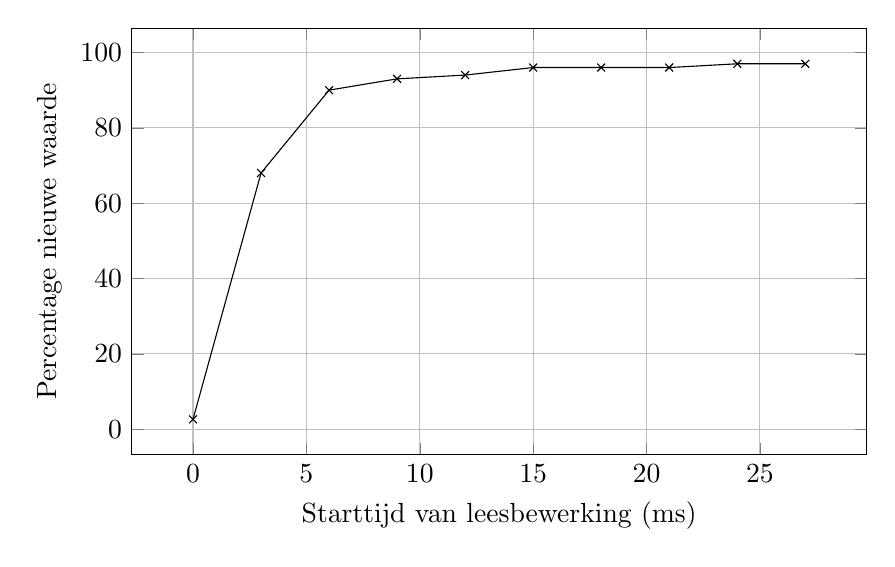
\begin{tikzpicture}
	
	\begin{axis}[
		xlabel={Starttijd van leesbewerking (ms)},
		ylabel={Percentage nieuwe waarde},
		domain = 0:1,
		grid = major,
		height=7cm,
		width=.9\textwidth
	]
	

	\addplot[color=black,mark=x]
	        plot coordinates {
	       		(0, 2.6)
				(3, 68)
				(6,90)
				(9,93)
				(12,94)
				(15,96)
				(18,96)
				(21,96)
				(24,97)
				(27,97)
	        };

	\end{axis}
\end{tikzpicture}
\caption{Consistentie: Percentage van de queries dat op een gegeven tijdstip de juiste data leest voor HBase. Het gemiddelde verschil tussen het starten en stoppen van het lezen op een willekeurig record is ongeveer 6ms, in het geval van hetzelfde record kan dit significant langer duren. }
\label{fig:consistentie-hbase-correct}
\end{figure}


\begin{figure}[tb!]
	\begin{minipage}{0.5\textwidth} 
	\textbf{Schrijven}
	\begin{enumerate}
	\item Lock de rij(en), om te beschermen tegen concurrente schrijfacties. 
	\item Haal het huidige schrijfnummer op
	\item Voeg aanpassingen toe aan WAL (Write Ahead Log)
	\item Pas aanpassing toe op de Memstore (cache geheugen)
	\item Commit de transactie, m.a.w. zet het leespunt op het nieuwe schrijfnummer
	\item Unlock de rijen
	\end{enumerate}
	\end{minipage} \hfill
	\begin{minipage}{0.3\textwidth} 
	\textbf{Lezen}
	\begin{enumerate}
	\item Open de lezer
	\item Ga naar het huidige leespunt
	\item Filter al de KeyValues paren met schrijfnummer > leespunt
	\item Sluit de lezer
	\end{enumerate}
	\end{minipage}
	\caption{HBase: Het vereenvoudigde lees- en schrijfmodel voor strikte consistentie in HBase naar Lars Hofhansl\cite{hbase-acid}}\label{fig:consistency-hbase-uitleg}
\end{figure}

\paragraph{MongoDB} MongoDB biedt strikte consistentie aan als er van de primary gelezen wordt maar er zijn ook andere schrijf- en leesmethodes. Een verschil met HBase is dat het bij alle mogelijke lees- en schrijfmethodes mogelijk is om de nieuwe data al te lezen vooraleer de schrijfbewerking beëindigd is. Een schrijfbewerking wacht op de server nog na het schrijven en vrijgeven van zijn schrijf lock. Een verklaring is hiervoor niet gevonden.

Uit figuren \ref{fig:consistentie-mongodb-primary}, \ref{fig:consistentie-mongodb-primarypreferred}, \ref{fig:consistentie-mongodb-secondary}, \ref{fig:consistentie-mongodb-secondarypreferred} en \ref{fig:consistentie-mongodb-nearest} kan een analyse gemaakt worden hoeveel kans er is dat een leesbewerking de nieuwe data al zal lezen. Voor lezer 1 tot 5, dit zijn tijdstippen 0, 2, 4, 6 en 8 ms, is een kans berekend ten opzichte van het starttijdstip. Een figuur is getekend voor 4 leesconfiguraties in plot \ref{fig:consistentie-mongodb-correct}. 

Uit figuren \ref{fig:consistentie-mongodb-verschillende-schrijfacties} blijkt dat er geen significant verschil is tussen de leesacties onder verschillende schrijfgaranties, indien men de starttijdstippen vergelijkt. De schrijfconfiguraties geven geen garanties tijdens het uitvoeren maar enkel na de voltooiing van de schrijfoperatie.  

Uit tabel \ref{table:consistentie-mongodb-inconsistency} blijkt dat het in MongoDB niet is gegarandeerd dat als een lezer de nieuwe waarde leest, dat al de overige lezers dat ook zullen doen. In dit geval was het schrijven nog niet voltooid en een bepaalde lezer leest de nieuwe data al. Maar een bewerking die later gestart is, leest de oude waarde nog. Dit kan verklaard worden doordat het verschillende servers zijn waarop gelezen wordt. In dit geval waren het verschillende lezers en dus verschillende gebruikers, maar de MongoDB driver controleert periodiek welke server het dichtste bij is. Dit controle kan tussen deze 2 bewerkingen gebeuren en men kan van een andere instantie lezen (in het geval de leesconfiguratie niet op primary staat). Er is bij MongoDB géén garantie op monotone leesbewerkingen. 

Aangezien er in de testomgeving een uniforme netwerkvertraging is naar alle instanties, volgt de data de veronderstelling dat de dichtstbijzijnde node in iets minder 1/3 van de gevallen een primary is en iets meer dan 2/3 een secondary. Met 5\% afwijking is het moeilijk te stellen dat deze significant is. 

Tenslotte hebben primary en primary-preferred in deze testen geen significante verschillen. Dit komt omdat de primary heel de tijd beschikbaar is. 

\begin{table}
\centering
\begin{tabular}{l | l l l l}
Lezer & Start lezen (ms) & Stop lezen (ms) & Gelezen waarde & Correct? \\
\hline
\multirow{2}{*}{1} & 2,200 & 3,213 & 12553\textbf{3}813315 & Nee\\
 & 13,426 & 14,279 & 12553\textbf{4}813315 & Ja \\
 \multirow{2}{*}{3} & 17,458 & 18,834 & 12553\textbf{3}813315 & Nee\\
 & 29,063 & 29,897 & 12553\textbf{3}813315& Ja \\
\end{tabular}
\caption{Consistentie: Ruwe data van MongoDB test waarbij inconsistente data wordt gelezen na het lezen van consistente data op verschillende lezers met het lezen via nearest en schrijven via fsync\_safe}
\label{table:consistentie-mongodb-inconsistency}
\end{table}


\begin{figure}[!htf]

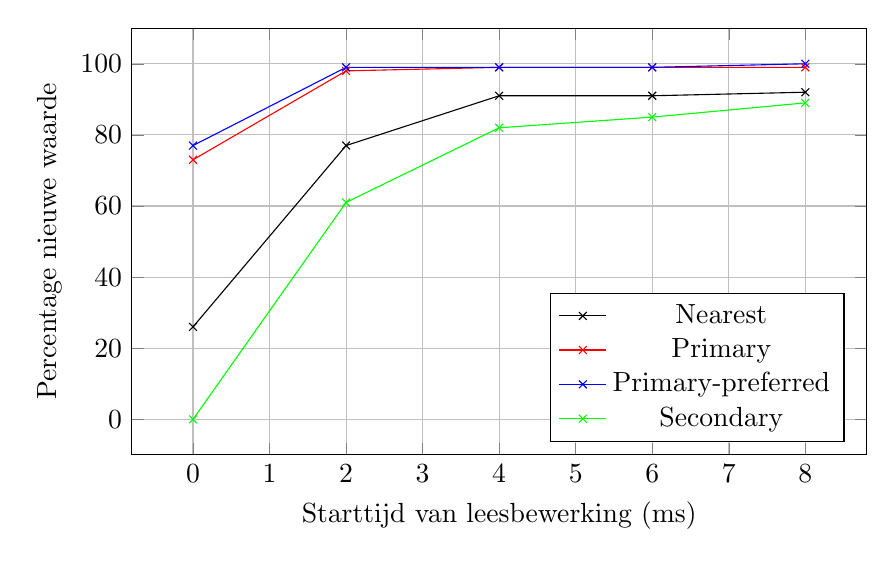
\begin{tikzpicture}
	
	\begin{axis}[
		xlabel={Starttijd van leesbewerking (ms)},
		ylabel={Percentage nieuwe waarde},
		domain = 0:1,
		grid = major,
		height=7cm,
		width=.9\textwidth,
		legend pos= south east
	]
	
	\addplot[color=black,mark=x]
	        plot coordinates {
	       		(0, 26)
				(2, 77)
				(4,91)
				(6,91)
				(8,92)
	        };
	\addlegendentry{Nearest}

	\addplot[color=red,mark=x]
	        plot coordinates {
	       		(0, 73)
				(2, 98)
				(4,99)
				(6,99)
				(8,99)
	        };
	\addlegendentry{Primary}
	
	\addplot[color=blue,mark=x]
      plot coordinates {
	       		(0, 77)
				(2, 99)
				(4,99)
				(6,99)
				(8,100)
      };
	\addlegendentry{Primary-preferred}
	
	\addplot[color=green,mark=x]
   plot coordinates {
	       		(0, 0)
				(2, 61)
				(4,82)
				(6,85)
				(8,89)
   };
	\addlegendentry{Secondary}
	\end{axis}
\end{tikzpicture}
\caption{Consistentie: Percentage van de queries dat van de eerste keer juist de data leest bij 0ms, 2ms, 4ms, 6ms en 8ms voor MongoDB. De gemiddelde vertraging op een onafhankelijke leesoperatie is 1ms. }
\label{fig:consistentie-mongodb-correct}
\end{figure}


\paragraph{Conclusie} Beide database systemen bieden strikte consistentie aan maar hebben een verschillende uitwerking hiervan: bij HBase worden de leesoperaties uitgesteld tot de volledige voltooiing van de schrijfoperatie, bij MongoDB zal de data al vroeger beschikbaar zijn. Beide systemen zijn \textit{session} consistent, \textit{read-your-own-write} en monotoon consistent, indien er bij MongoDB op een primary wordt gelezen.  

\textit{Session}, \textit{read-your-own-write}, \textit{casual} en \textit{monotonic} consistentie zijn niet gegarandeerd in MongoDB indien er niet gelezen wordt op een primaire. De MongoDB driver kan op ieder moment een andere server kiezen in deze gevallen en kan dus nog oude data lezen. 

Een hypothese is dat bij MongoDB het falen van de primary de consistentie garanties zal beïnvloeden, een nieuwe primary kan verkozen worden. Wanneer geen enkele secondary deze update al heeft ontvangen, zou deze dus verloren gaan. Maar een gebruiker zou de data al van de oude primary gelezen kunnen hebben, in dit geval faalt hier de stikte consistentie. Dit gedrag is wel niet getest en bevestigd. HBase heeft deze situatie niet door de keuze om de leesbewerking te verlengen, een gebruiker dient dus langer te wachten op zijn data. 

\section{Conclusie}
De drie systemen hebben verschillende aanpak naar beschikbaarheid en consistentie. Pgpool-II is het minst geavanceerd systeem door geen automatisch herstel te ondersteunen, maar door de centrale aanpak van de routernode heeft dit systeem geen netwerk verkeer als het niet wordt gebruikt. 

MongoDB is een systeem dat weinig configureerbaar is naar het gedrag bij het falen van een instantie, daarentegen zijn er een verschillende configuratiemogelijkheid naar het lees- en schrijfgedrag. Enkel als er gelezen wordt van de primary, zal er strikte consistentie zijn. Het is nog onduidelijk welke garanties er zijn bij het falen van een primary. In normale situaties is het mogelijk om de nieuwe data snel te lezen. 

HBase is met behulp van Zookeeper configureerbaar naar het gedrag bij falen van een enkele instantie. De onbeschikbaarheidsperiode kan verkleind of vergroot worden. De consistentiegaranties van HBase zijn strikt voor een enkel record maar dit komt wel voor een prijs: een leesactie wordt uitgesteld indien er een de schrijfactie op dat record uitgevoerd wordt. 